\documentclass{book}

\usepackage{libertine}

\usepackage{graphicx}
\graphicspath{ {images/} }
\usepackage{listings}
\usepackage{color}
\usepackage{tikz}
\definecolor{mygreen}{rgb}{0,0.6,0}
\definecolor{gray}{rgb}{0.4,0.4,0.4}
\definecolor{darkblue}{rgb}{0.0,0.0,0.6}
\definecolor{cyan}{rgb}{0.0,0.6,0.6}
\usepackage[top=3cm, bottom=2cm, outer=3cm, inner=2.1cm, headsep=14pt]{geometry}
\newcommand{\shrug}[1][]{%
	\begin{tikzpicture}[baseline,x=0.8\ht\strutbox,y=0.8\ht\strutbox,line width=0.125ex,#1]
	\def\arm{(-2.5,0.95) to (-2,0.95) (-1.9,1) to (-1.5,0) (-1.35,0) to (-0.8,0)};
	\draw \arm;
	\draw[xscale=-1] \arm;
	\def\headpart{(0.6,0) arc[start angle=-40, end angle=40,x radius=0.6,y radius=0.8]};
	\draw \headpart;
	\draw[xscale=-1] \headpart;
	\def\eye{(-0.075,0.15) .. controls (0.02,0) .. (0.075,-0.15)};
	\draw[shift={(-0.3,0.8)}] \eye;
	\draw[shift={(0,0.85)}] \eye;
	% draw mouth
	\draw (-0.1,0.2) to [out=15,in=-100] (0.4,0.95); 
	\end{tikzpicture}}
\lstdefinestyle{customcs}{
	frame=single,
	basicstyle=\footnotesize\ttfamily, 
	tabsize=2, 
	extendedchars=true, 
	breaklines=true, 
	stringstyle=\color{red}\ttfamily, 
	showspaces=false, 
	showtabs=false, 
	commentstyle=\color{gray},
	morecomment=[l]{//},
	morecomment=[s]{/*}{*/},
	showstringspaces=false, 
	morekeywords={  abstract, event, new, struct,
		as, explicit, null, switch,
		base, extern, object, this,
		bool, false, operator, throw,
		break, finally, out, true,
		byte, fixed, override, try,
		case, float, params, typeof,
		catch, for, private, uint,
		char, foreach, protected, ulong,
		checked, goto, public, unchecked,
		class, if, readonly, unsafe,
		const, implicit, ref, ushort,
		continue, in, return, using,
		decimal, int, sbyte, virtual,
		default, interface, sealed, volatile,
		delegate, internal, short, void,
		do, is, sizeof, while,
		double, lock, stackalloc,
		else, long, static,
		enum, namespace, string, var},
	keywordstyle=\color{blue},
	identifierstyle=\color{cyan},
}

\lstdefinestyle{customc}{
	basicstyle=\ttfamily,
	columns=fullflexible,
	showstringspaces=false,
	commentstyle=\color{gray}\upshape,
	belowcaptionskip=1\baselineskip,
	breaklines=true,
	frame=single,
	xleftmargin=\parindent,
	language=C,
	showstringspaces=false,
	basicstyle=\footnotesize\ttfamily,
	keywordstyle=\bfseries\color{blue},
	commentstyle=\itshape\color{gray},
	identifierstyle=\color{black},
	stringstyle=\color{red},
}

\lstdefinelanguage{XML}
{
	morestring=[b]",
	morestring=[s]{>}{<},
	morecomment=[s]{<?}{?>},
	stringstyle=\color{black},
	identifierstyle=\color{darkblue},
	keywordstyle=\color{cyan},
	morekeywords={xmlns,version,type}% list your attributes here
}

\lstdefinestyle{custombash}
{
	frame=single,
	basicstyle=\footnotesize\ttfamily,
	columns=fullflexible,
	showstringspaces=false
}

\lstdefinestyle{customxml}
{
	frame=single,
	basicstyle=\footnotesize\ttfamily,
	columns=fullflexible,
	showstringspaces=false
}

\begin{document}

\author{BlackCentipede}
\title{Advanced C\# for Low-Level Programming\\
	   \large Licensed Attribution-NonCommercial 3.0 
	   \\United States (CC BY-NC 3.0 US) \\
   	   \small https://creativecommons.org/licenses/by-nc/3.0/us/}
\date{November 2018}

\frontmatter

\maketitle
\newpage
\large Book Contributors \newline
\begin{itemize}
	\item Jamesbascle - For grammar correction.
\end{itemize}

\newpage
\tableofcontents

\mainmatter
\chapter{Introduction}
\section{What you will need to get started}
You will need Dotnet Core and Clang/LLVM compilers installed for this book. The book will assume you are working on Linux platform although knowledge gained here can be applied on any other platforms including Windows.

You can install Dotnet Core SDK from this URL which contains an instruction to install Dotnet Core on your respective distribution:
\newline \newline
 https://www.microsoft.com/net/download/linux
\newline \newline
Clang/LLVM Compilers can be installed or compiled on your respective linux distribution, the table below will get you started.
\newline \newline
\begin{tabular}{| c | c |}
	\hline 
	\textbf{Linux Distribution} & \textbf{Command Line or Link} \\
	\hline
	 Arch Linux & pacman -S llvm clang  \\
	 \hline
	 Ubuntu & apt.llvm.org/ \\
	 \hline
	 Debian & apt.llvm.org/ \\
	 \hline
	 Red Hat Enterprise Linux & developers.redhat.com/blog/2018/07/07/yum-install-gcc7-clang/ \\
	 \hline
	 Fedora & dnf install llvm clang \\
	 \hline
	 CentOS & Compile LLVM/Clang yourself  \shrug \\
	 \hline
	 OpenSUSE & zypper install llvm clang \\
	 \hline
	 Gentoo Linux & https://wiki.gentoo.org/wiki/Clang \\
	 \hline
	 Slackware Linux & Compile LLVM/Clang yourself  \shrug \\
	 \hline
\end{tabular}

\section{Minimum Knowledge}
You'll need to have some comprehension of C\# and C languages before starting this book though this book will try to walk you through the basic of C/C++.

\chapter{Introduction to P/Invoke}

\section{Getting Started}
First, create a Directory as 'ChapterTwo' for this project and create a new file, 'ChapTwo.c' under 'ChapterTwo' folder.

Let's assume we have a basic Addition function in a C Library that we want to call.

\lstinputlisting[style=customc, language=C]{codes/Chap2/Chap2Snippet1.c}

It's a simple Addition Operation at a first glance, but there are\newline considerations that must be observed first before attempting to write platform invocation wrapper code for the function above:

\begin{enumerate}
	\item \label{itm:first} `int` datatype in C can be considered 2 bytes long or 4 bytes long or however long it may be depending on the architecture and compiler that the library is compiled on. In C Standard, int must be capable of containing \textbf{at least} the [\textminus32,767, +32,767] range; thus, it is at least 16 bits in size.
	
	\item Due to \ref{itm:first}, you can reasonably safeguard against data loss by substituting C\# Int32(int) which contains 4 bytes or you may choose follow the standard strictly by supplying C\# Int16(short) which contains 2 bytes, even though it can suffer data loss. The best approach is to avoid using "at least" integers in C and instead use fixed size integers provided by the compiler in ''stdint.h'' header if you have Foreign Function Interface kept in mind.
	
	\item Sometimes you have to keep Endianess in mind although it is less of a concern in x86\_64 architecture since little endianess is the default.
\end{enumerate}
The best approach to writing the Addition function is to make it clear what sized integers you're attempting to add  if possible.

\lstinputlisting[style=customc, language=C]{codes/Chap2/Chap2Snippet2.c}

\section{Compiling the Library}
This book assumes you have sufficient knowledge of C, we will still however, provide compilation instruction. The following command assumes that you have named your source code file as 'ChapTwo.c' as instructed at the beginning of this chapter.

\lstinputlisting[style=custombash,language=Bash]{codes/Chap2/Chap2Snippet3.sh}

Here we examine and explain the compiler arguments:

\begin{enumerate}
	\item '-std=c99' specify that we are compiling C source code under C99 Standard.
	\item '-shared' specify that we want the program to be compiled as shared/dynamic library.
	\item '-fPIC' specify that code must be position independent so that the resultant library can be loaded by other processes and have code be made available to be run anywhere in program address space regardless of code's address.
	\item '-olibChapTwo.so' specify what the output library should be named. lib prefix in 'libChapTwo.so' is a matter of naming convention to be followed on Linux although compilers like clang and gcc do search libraries based on lib prefix when using '-l' option. 
\end{enumerate}
\newpage
\section{Configuring C\# Project}
Since we're already in "ChapterTwo" directory, we can go ahead and run 'dotnet new Console'. There are a few steps we need to take to add the C code to our C\# project. First, we need to automate the compilation process of our C file and copy the compiled C library to the target directory for Debug, Release, or any other configurations.

Open up 'ChapterTwo.csproj' file with your favorite editor, and add the following under '</PropertyGroup>' inside '<Project>' tag.

\lstinputlisting[style=customxml, language=XML]{codes/Chap2/Chap2Snippet4.xml}

The snippet above does few things after building our C\# project:
\begin{enumerate}
	\item Compile ChapTwo.c code as a shared library, libChapTwo.so
	\item Copy libChapTwo.so into any target directory that C\# is being built in.
\end{enumerate}

This makes it significantly easier to modify our code without having to run any additional commands for it to take effect.

Your CSProj should look like the following:

\lstinputlisting[style=customxml, language=XML]{codes/Chap2/Chap2Snippet5.xml}
\newpage
\section{Wrapping C Code in C\#}
Open up Program.cs, add a new using directive at the top of your source code.

\lstinputlisting[style=customcs]{codes/Chap2/Chap2Snippet6.cs}

This line imports all of the platform invocation services which enables us to interact with our C library with ease.

Add the following lines under Program class:

\lstinputlisting[style=customcs]{codes/Chap2/Chap2Snippet7.cs}

The DllImport attribute declares that a static externally defined function is defined in a C library and to have CLR create a Platform Invocation stub to define the said function within external library.

It is required to declare the function with static and extern modifiers since it is a function that is both independent of state and externally defined.

Finally, modify the ''Console.WriteLine'' line to the following:

\lstinputlisting[style=customcs]{codes/Chap2/Chap2Snippet8.cs}
And your source code should look as follows:

\lstinputlisting[style=customcs, language={[Sharp]C}]{codes/Chap2/Chap2Snippet9.cs}
\newpage
Finally, your program is ready to be executed. You can run:
\lstinputlisting[style=custombash,language=Bash]{codes/Chap2/Chap2Snippet10.sh}

And we have the following:

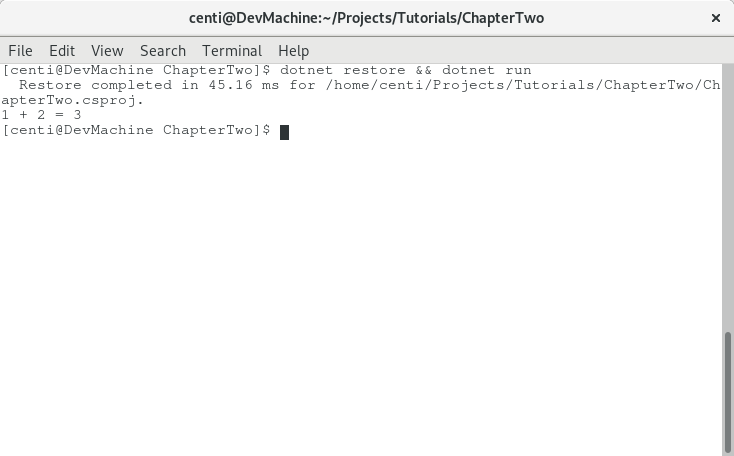
\includegraphics[width=\textwidth]{ChapTwoConsole}
It works as expected!
\newpage
\section{Some Backgrounds}
There are few things happening when a function with DllImport is called, if this is the first time the function is being called, the Runtime will first load the external library immediately, then load the symbol ''Sum'' when P/Invoke defined method is called, and finally generate a P/Invoke stub for that function to support the call to the external function.

The symbol is merely just that, a symbol that is exported by C Library that can be resolved to an address to where code or variable is located. You can find a list of symbols by running ''objdump -T libChapTwo.so'' on your library and you'll have the following:
\newline \newline
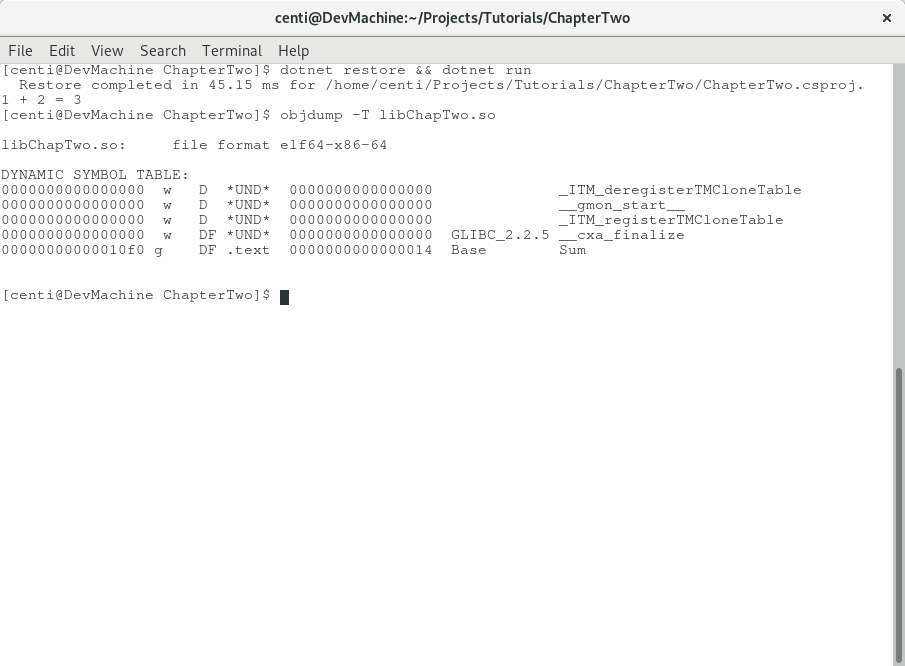
\includegraphics[width=\textwidth]{ChapTwoConsoleTwo}
\newline\newline
You will notice that the Add symbol is shown in the symbol table in your library, this is how the CLR looks up a function by entry name.
\chapter{Introduction to Pointer}
\section{Overview on Pointer}
If you already have sufficient understanding about Pointer in both C\# and C languages, you can skip this chapter. This chapter is for introducing beginners to the concept of pointer.

A pointer is essentially an address to an area of memory. You can represent what that pointer is supposed to be such as a pointer of integer, struct, classes, function or even another pointer.
To read and write memory that pointer is pointing to, you have to first dereference that pointer and you can do so by using asterisk in front of a pointer variable to dereference it, not to be confused with multiplication operator.

\lstinputlisting[style=customc, language=C]{codes/Chap3/Chap3Snippet1.c}
\newpage
The C snippet above first allocate with malloc function a new buffer of memory up to a size of int32\_t datatype and return a void* pointer which then get casted into int32\_t* pointer type. You can access the pointer in two ways, writing it similar fashion as you would when accessing an array and to use '*' operator to dereference the pointer to read and write the first datatype the pointer is currently pointing to.

Let's get started by creating a new "ChapterThree" directory and create a new file, "ChapThree.c" and open with your favorite editor.

We will need three headers to provide the functionalties and types we need for this chapter.

\lstinputlisting[style=customc, language=C]{codes/Chap3/Chap3Snippet2.c}

Let's declare a main function that allocate a buffer of 20 integers and return a pointer address to that buffer and we'll treat it as an array of integer.

\lstinputlisting[style=customc, language=C]{codes/Chap3/Chap3Snippet3.c}
\newpage
The output would be shown as this:

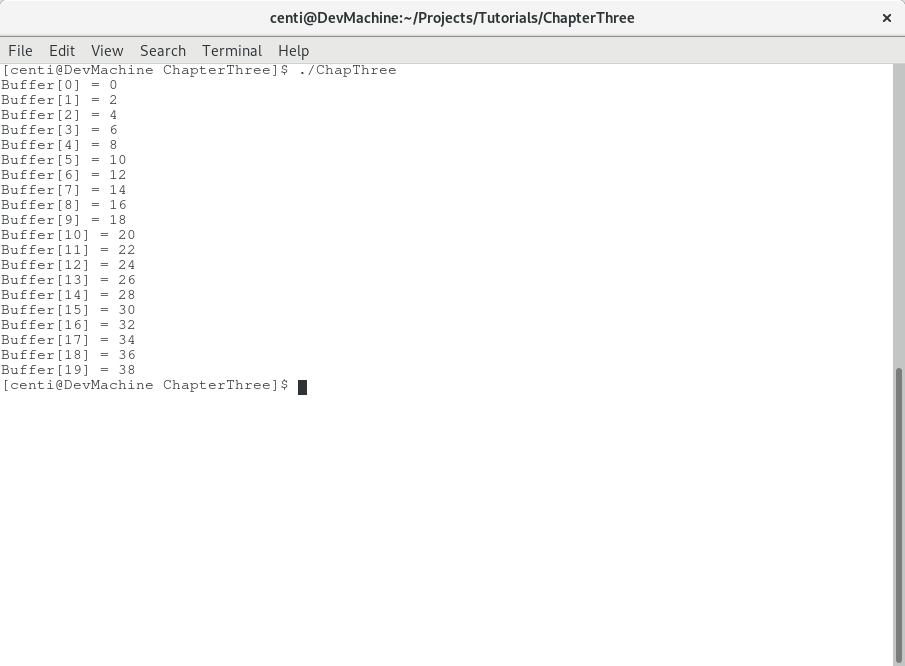
\includegraphics[width=\textwidth]{ChapThreeConsole}
\newpage
There are few things that may be confusing in the snippet above and why it is an acceptable practice in C:

\begin{enumerate}
	\item When you use malloc to allocate buffer, malloc keeps a record of how big the block of memory is so that it can be freed in later time, however you cannot and should not access that size information within malloc, keeping track of buffer size is your responsibility.
	
	\item When using malloc, you allocate the amount of data you would need by using sizeof keyword to determine how many bytes capacity you need in a buffer to cover that information and you can multiply that element size by the number of elements you want allocated for your program. In the snippet above, size of int32\_t type would resolves to 4 and then multiplied by 20, so we would have a buffer that have the capacity to hold 20 int32\_t elements.
	
	\item Malloc does not zero out the memory by default and in this specific case shown above, it's much more efficient since it's not necessary to zero out the memory since whatever memory/value stored in that allocated memory would be modified immediately after allocating. It however important that you need to zero out or assign a value to the memory otherwise when you attempt to read the said memory it would present an undefined behavior since you can't alway be sure the program will behave consistently when there are random value stored in the allocated memory and being processed by the program.
\end{enumerate}

Because of the fact behind malloc/free that LibC does store information about the pointer that is allocated with those functions, it discouraged to use different library or framework to free that memory, although most library and framework may likely use the same functions.
\newpage
\section{The Function Pointers}
Function pointers are a bit of a tongue twister, because the way it is defined in C can be confusing.

\lstinputlisting[style=customc, language=C]{codes/Chap3/Chap3Snippet4.c}

The snippet above is a declaration of function pointer for a function that returns a int32\_t after accepting two int32\_t parameters. It currently pointing at nothing and would cause segmentation fault when you attempt to call it, so you have to assign a function for it to be used.

One example of this use case is that we can dynamically modify the behavior of our program during runtime and essentially allow our program to switch logic at different points during program execution like so:
\lstinputlisting[style=customc, language=C]{codes/Chap3/Chap3Snippet5.c}
\newpage
It would produce an output as followed:

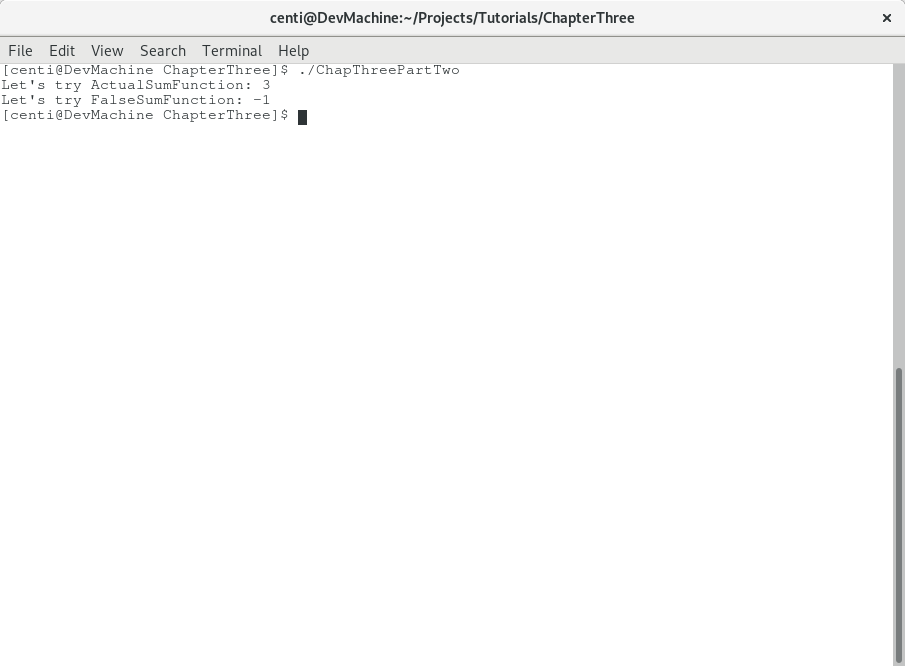
\includegraphics[width=\textwidth]{ChapThreeConsoleTwo}
\newpage
\section{C\# Counterpart}
C\# does support pointer in a similar fashion as C so long that the code blocks, methods, or types are defined with unsafe modifier. Those can be accomplished by using snippets below as a demonstration:
\lstinputlisting[style=customcs]{codes/Chap3/Chap3Snippet6.cs}
\lstinputlisting[style=customcs]{codes/Chap3/Chap3Snippet7.cs}
\lstinputlisting[style=customcs]{codes/Chap3/Chap3Snippet8.cs}

Though this is not required, you can use IntPtr and Marshal static class to accomplish everything of above.

When using \textbf{unsafe} modifier, compiler will throw an error unless you explicitly specify that you want to compile unsafe code. For CoreCLR, you can do so by adding the following into your csproj file inside the  <PropertyGroup> tags:

\lstinputlisting[style=customxml, language=XML]{codes/Chap3/Chap3Snippet9.xml}

Marshal static class from System.Runtime.InteropServices offer a variety of functions for marshaling pointers to usable data types and vice versa. You can also generate a function in runtime in CLR and pass it over to C program so that C program can use your newly created function during it's execution.

Passing a runtime generated function to C will be covered in Chapter 5.

\chapter{The History On Delegate Approach}
\section{Note}
It is recommended \textbf{not} to skip this chapter, because for the remainder of this book, this book will be making an extensive use of Advanced DL Support library. More information can be found here: https://github.com/Firwood-Software/AdvanceDLSupport

\section{Prior to Nov 2017}
There were at the time that variety of CLR implementations for C\# does not conform to the same behavior expected for P/Invoke. C\# at the time of writing does not have any way to reach the global variable through the normal DllImport attribute approach, and it has to be done by loading libdl and dlopen/dlsym/dlclose. Libdl is a library used to dynamically load external native libraries at runtime and you can retrieve the address to variables or functions by using dlsym which accepts the input for symbol.

In Mono, it would load the external native library with dlopen and you would be sharing the same instance for this external library when using dlopen/dlsym/dlclose. CoreCLR would load the library in other means than dlopen and that would create two instances of the same library which would reflect a different behavior.
\newpage
\section{Precursor to Advanced DL Support}
ADL, Advanced DL Support, was created shortly after Nov 2017 to work around the problem with P/Invoke and inconsistent behavior with different implementations of CLR. It was initially accomplished by doing the followings in concept:

\lstinputlisting[style=customcs]{codes/Chap4/Chap4Snippet1.cs}

But this is an extremely inefficient approach to wrap native libraries. Advanced DL Support utilizes CIL, Common Intermediate Language, the language that C\# compiles to, to generate new types and return new instances of said types for you to utilize native libraries which can be disposed, and therefore do no longer have to be kept around for the duration of the program runtime. You can create new types and code while the program is running and that is thank to the Just-In-Time Compiler. You supplement an interface, abstract class or even a base class to ADL to generate a new type at runtime that binds all of the functions and variables and make it significantly easier to bind native library at an equivalent speed to DllImport attribute approach.

\newpage
\section{The Advanced DL Support Approach}
Make sure you have a new directory created for Chapter 4 and run the following to initialize your Dotnet Console project:

\lstinputlisting[style=custombash, language=C]{codes/Chap4/Chap4Snippet2.sh}

We will need to both reference ''AdvancedDLSupport'' from Nuget and to add compilation target for C Library that we will be wrapping with for this demonstration.

Your CsProj file should looks like this:

\lstinputlisting[style=customxml, language=XML]{codes/Chap4/Chap4Snippet3.xml}

The C Library source could will simply have a global variable and a function to increment the said variable as followed:

\lstinputlisting[style=customc, language=C]{codes/Chap4/Chap4Snippet4.c}

For demonstration of ADL, the native library can be binded in C\# by simply creating an interface for library and it supports properties:

\lstinputlisting[style=customcs]{codes/Chap4/Chap4Snippet5.cs}
\newpage
The following output from the program will display as followed:

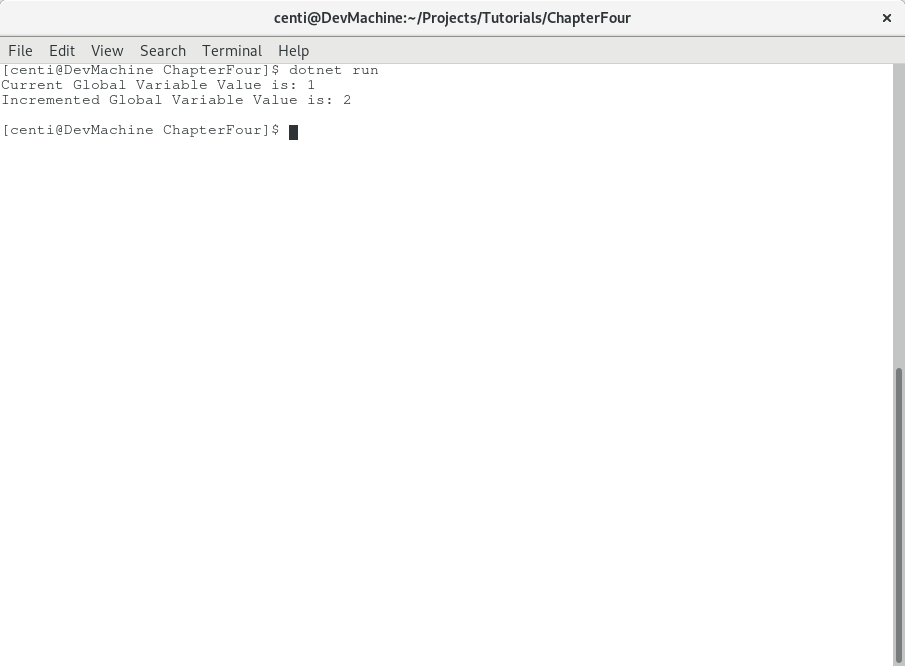
\includegraphics[width=\textwidth]{ChapFourConsole}

As you can tell, the amount of time saved in writing the binding for native library compared to both DllImport and the Delegate Approach are very significant. You simply only have to write an interface to the native library and that eliminates the need for writing DllImport attribute repeatingly and you can also access the global variable via properties.

\chapter{Embedding Mono}

\backmatter
% bibliography, glossary and index would go here.

\end{document}